\documentclass[oneside, 10pt]{book}

\usepackage{graphicx}
\usepackage{enumitem}

\usepackage{hyperref}
\hypersetup{
colorlinks  = True,
linkcolor= blue
}

\begin{document}
%\tableofcontents
%\listoffigures
%\listoftables
\chapter{Introduction}
Lorem ipsum dolor sit amet, consectetur adipiscing elit, sed do eiusmod tempor incididunt ut labore et dolore magna aliqua. Nunc sed id semper risus in hendrerit gravida rutrum quisque. Quam pellentesque nec nam aliquam. Lectus nulla at volutpat diam ut. Sed velit dignissim sodales ut eu sem.

\section{consectetur adipiscing elit}

Lorem ipsum dolor sit amet, consectetur adipiscing elit, sed do eiusmod tempor incididunt ut labore et dolore magna aliqua. 


\section{ eiusmod tempor incididunt}
Tincidunt vitae semper quis lectus nulla at volutpat diam. Cras pulvinar mattis nunc sed blandit libero volutpat. Netus et malesuada fames ac. Dictum non consectetur a erat nam at. 

In the section 1.1, we discuss something important. Now change the hard coded section value using cross referencing. 

\begin{equation}
\int f(x) dx  = \int x^3e^-{x} dx  
\end{equation}

In the Equation 1.1, we have found the integration of the function...


\begin{equation}
\frac{dy}{dx} = \sin ax \cos ax \frac{e^x}{\sum_{n=1}^{\infty} a_n f(x)}
\end{equation}

In the Equation 1.2, we discuss something. Omg, now my guide is telling me to keep this equation in section 1.1, how do I do that? Cross referencing will help me?


\chapter{Captioning, Labeling and Referering Figures}

\begin{figure}[htb!]
\centering
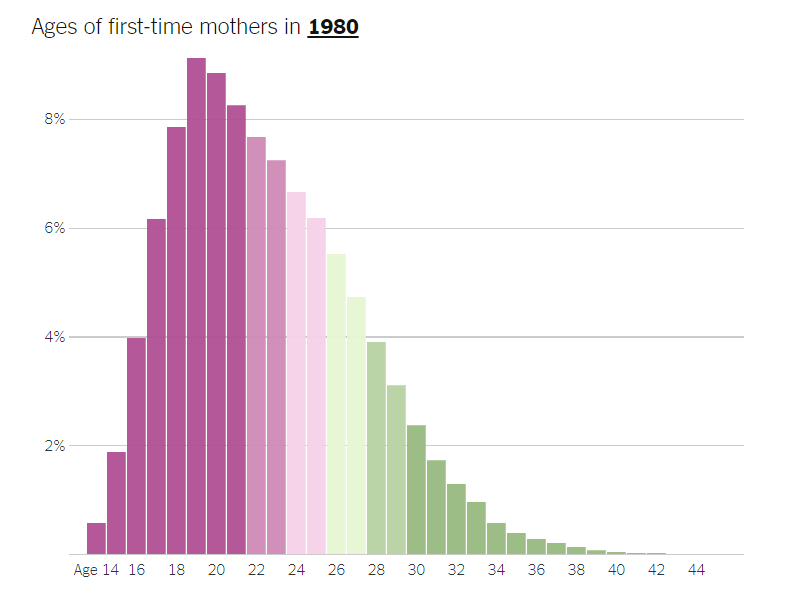
\includegraphics[scale=.4]{img/ages_first_mothers}
\caption{Ages of First Time Mothers in 1980}
\end{figure}

In the Figure 2.1, we can identify the distribution of the ages of the mothers in 1980. 

Ut tristique et egestas quis ipsum suspendisse. Volutpat odio facilisis mauris sit amet massa vitae tortor condimentum. Urna porttitor rhoncus dolor purus non enim. Adipiscing at in tellus integer.
\label{djfkdj}


\chapter{Captioning and Referring a Table}
In Chapter 2,  in Page 2 in the  Figure 2.1 we have discussed ages of the first time mothers and now we will see something else. 

\begin{table}[htb!]
\centering
\renewcommand*{\arraystretch}{1.25}
\begin{tabular}{ |p{3cm}|p{3cm}|p{3cm}|p{3cm}|  }
	\hline
	\multicolumn{4}{|c|}{\bf \large Country List} \\
	\hline
	Country Name     or Area Name& ISO ALPHA 2 Code &ISO ALPHA 3 Code&ISO numeric Code\\
	\hline
	Afghanistan   & AF    &AFG&   004\\
	Aland Islands&   AX  & ALA   &248\\
	Albania &AL & ALB&  008\\
	Algeria    &DZ & DZA&  012\\
	American Samoa&   AS  & ASM&016\\
	Andorra& AD  & AND   &020\\
	Angola& AO  & AGO&024\\
	\hline
\end{tabular}
\caption{List of Countries and its ISO Alpha Code}
\end{table}

In the Table 3.1, we have discussed list of countries and its iso alpha code. 

LaTeX provides several packages for designing the layout:
\begin{enumerate}[label={(P\arabic*)}]
	\item geometry
	\item typearea
	\item fancyhdr
	\item scrpage2
	\item setspace
\end{enumerate}

The package mentioned in (P3) is very important in the life. 
\chapter{Conclusion}

In Chapter 1, we have learnt something, In Chapter 2 at the page 2 we have learnt something else. Finally in chapter 3, in the Table 3.1, we have learnt how to label the table also. 

As given in the Equation 1.1, in the Page 1, we can check for some thing \dots



\end{document}